\documentclass{standalone}
\usepackage{tikz}
\usepackage{pgfplots}
\pgfplotsset{compat=1.18}
\begin{document}

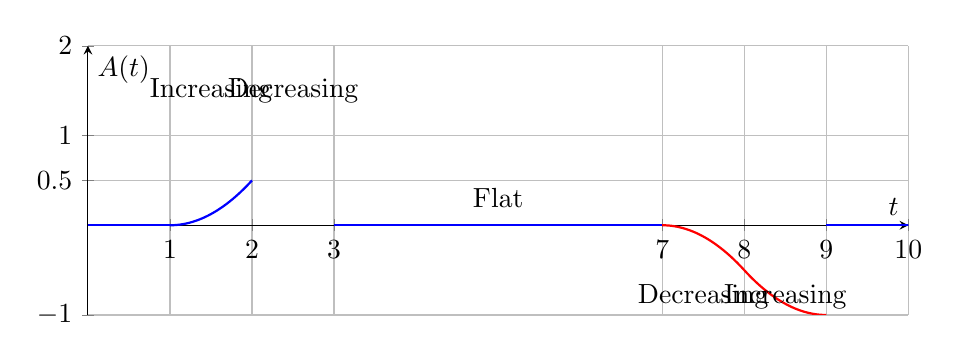
\begin{tikzpicture}[scale=1]
\begin{axis}[
    domain=0:10,
    samples=200,
    axis lines=middle,
    xlabel={$t$},
    ylabel={$A(t)$},
    ymin=-1,
    ymax=2,
    xtick={0,1,2,3,7,8,9,10},
    ytick={-1,0,0.5,1,2},
    width=12cm,
    height=5cm,
    grid=both,
]

% 0 to 1
\addplot[blue,thick,domain=0:1] {0};

% 1 to 2
\addplot[blue,thick,domain=1:2] {0.5*x^2 - x + 0.5};

% 2 to 3
\addplot[blue,thick,domain=2:3] {-0.5*x^2 + 3*x -1.5};

% 3 to 7
\addplot[blue,thick,domain=3:7] {0};

% 7 to 8
\addplot[red,thick,domain=7:8] {-0.5*x^2 + 7*x -24.5};

% 8 to 9
\addplot[red,thick,domain=8:9] {0.5*x^2 - 9*x + 39.5};

% 9 to 10
\addplot[blue,thick,domain=9:10] {0};

% Labels
\node at (axis cs:1.5,1.5) {Increasing};
\node at (axis cs:2.5,1.5) {Decreasing};
\node at (axis cs:5,0.3) {Flat};
\node at (axis cs:7.5,-0.8) {Decreasing};
\node at (axis cs:8.5,-0.8) {Increasing};

\end{axis}
\end{tikzpicture}

\end{document}

